%% BioMed_Central_Tex_Template_v1.06

% additional documentclass options:
%  [doublespacing]
%  [linenumbers] put the line numbers on margins

% uncomment this for twocolumn layout and comment line below
\documentclass[twocolumn]{bmcart}
% \documentclass{bmcart}

\usepackage{amsthm}
\usepackage{amsmath}
\usepackage{amssymb}
%\RequirePackage{natbib}
%\RequirePackage[authoryear]{natbib}% uncomment this for author-year bibliography
%\RequirePackage{hyperref}
\usepackage[utf8]{inputenc} %unicode support
%\usepackage[applemac]{inputenc} %applemac support if unicode package fails
%\usepackage[latin1]{inputenc} %UNIX support if unicode package fails

\usepackage{url}
% \usepackage{tabu}
% \usepackage{caption}
% \usepackage{booktabs}
% \usepackage{amsmath}
\usepackage{graphicx}
% \usepackage{caption}
% \usepackage{textcomp}
% \usepackage{subcaption}
% \usepackage{amssymb}
% \usepackage{multicol}
% \usepackage{authblk}
% \usepackage{sectsty}
% \usepackage[margin=20mm]{geometry}

% If you wish to display your graphics for your own use using includegraphic or includegraphics,
% then comment out the following two lines of code.
% These line *must* be included when submitting to BMC.
% All figure files must be submitted as separate graphics through the BMC submission process,
% not included in the submitted article.
% \def\includegraphic{}
% \def\includegraphics{}

% Put your definitions there:
\startlocaldefs
\endlocaldefs

\begin{document}

% Start of article front matter
\begin{frontmatter}
\begin{fmbox}
\dochead{Research}

\title{Bayesian decoding and confidence estimation for deep combinatorial sequence indexing with Pheniqs}

\author[addressref={aff1}, email={lg1883@nyu.edu}]{
    \inits{LG}
    \fnm{Lior}
    \snm{Galanti}
}
\author[addressref={aff2}, email={shasha@courant.nyu.edu}]{
    \inits{DS}
    \fnm{Dennis}
    \snm{Shasha}
}
\author[addressref={aff1}, corref={aff1}, email={kcg1@nyu.edu}]{
    \inits{KCG}
    \fnm{Kristin C}
    \snm{Gunsalus}
}
\address[id=aff1] {
    \orgname{Center for Genomics \& System Biology, Department of Biology, New York University},
    \street{12 Waverly Place},
    \postcode{10003}
    \city{New York},
    \cny{United States}
}
\address[id=aff2] {
    \orgname{Courant Institute, Department of Computer Science, New York University},
    \street{251 Mercer St},
    \postcode{10012}
    \city{New York},
    \cny{United States}
}

% Enter short notes here
% Short notes will be after addresses on first page.
% \begin{artnotes}
% \note{Sample of title note}     % note to the article
% \note[id=n1]{Equal contributor} % note, connected to author
% \end{artnotes}


% \end{fmbox}% comment this for two column layout
\begin{abstractbox}
\begin{abstract}
\parttitle{Background}
Systems biology increasingly relies on deep sequencing with combinatorial index tags called barcodes to associate individual biological sequences with their respective sample, individual cell, and/or molecule. Accurate data interpretation critically depends on discerning the correct origin of each sequence of interest, and hence on the confidence of the final classification confidence. This, in turn, is cumulatively impacted by the decoding confidence of the various barcodes. Preserving a classification quality score is especially desirable when the decision to assign or discard a read depends on factors only available downstream. These may include the observed distribution of expected barcodes within a mixture of bulk sequencing samples, or the number of individual cells that can be reliably detected in single-cell sequencing experiments. Despite these advantages, computation and reporting of decoding confidence scores have not been widely adopted. To improve overall performance at this critical stage of sequence analysis, we have developed a flexible and robustly engineered software package, Pheniqs, that supports arbitrarily complex barcoding schemes and enables standardized reporting of decoded index sequences with classification confidence scores.

\parttitle{Results}
Pheniqs implements both a standard minimum distance decoder and a probabilistic decoder that classifies sequence reads based on the full posterior probability of observed barcode indexes. Pheniqs consults basecalling quality scores and prior distributions to compute the posterior decoding error probability of individual barcodes and reports the resulting barcode sequences and confidence scores in standardized SAM auxiliary tags. Pheniqs can be extended with new error models and relies on intuitive confidence thresholds for fine-tuning decoding accuracy. Performance evaluation using synthetic data indicates that Pheniqs achieves greater accuracy than simple MDD or maximum likelihood estimation by correctly computing the full posterior classification probability. An optimized multi-threaded implementation assures that Pheniqs is both faster and scales better with large and complex barcode sets than existing tools.

\parttitle{Conclusions}
Using full posterior probabilities to decode barcodes with Pheniqs is faster and more accurate than existing tools, especially those who depend on minimum distance. With the availability of an efficient implementation and the increased reliance on combinatorial barcode for classification we encourage the community to switch to more accurate probabilistic methods.

\end{abstract}

%%%%%%%%%%%%%%%%%%%%%%%%%%%%%%%%%%%%%%%%%%%%%%
%%                                          %%
%% The keywords begin here                  %%
%%                                          %%
%% Put each keyword in separate \kwd{}.     %%
%%                                          %%
%%%%%%%%%%%%%%%%%%%%%%%%%%%%%%%%%%%%%%%%%%%%%%

\begin{keyword}
\kwd{demultiplex}
\kwd{barcode}
\kwd{confidence}
\end{keyword}

% MSC classifications codes, if any
%\begin{keyword}[class=AMS]
%\kwd[Primary ]{}
%\kwd{}
%\kwd[; secondary ]{}
%\end{keyword}

\end{abstractbox}
\end{fmbox}% uncomment this for twcolumn layout
\end{frontmatter}

%%%%%%%%%%%%%%%%%%%%%%%%%%%%%%%%%%%%%%%%%%%%%%
%%                                          %%
%% The Main Body begins here                %%
%%                                          %%
%% Please refer to the instructions for     %%
%% authors on:                              %%
%% http://www.biomedcentral.com/info/authors%%
%% and include the section headings         %%
%% accordingly for your article type.       %%
%%                                          %%
%% See the Results and Discussion section   %%
%% for details on how to create sub-sections%%
%%                                          %%
%% use \cite{...} to cite references        %%
%%  \cite{koon} and                         %%
%%  \cite{oreg,khar,zvai,xjon,schn,pond}    %%
%%  \nocite{smith,marg,hunn,advi,koha,mouse}%%
%%                                          %%
%%%%%%%%%%%%%%%%%%%%%%%%%%%%%%%%%%%%%%%%%%%%%%

\section*{Background}
% The Background section should explain the relevant context and the specific issue that the software described is intended to address.

High-throughput sequencing with multiplexed sample barcodes is now standard practice, and single-cell applications are rapidly gaining in popularity. To enhance resolution and to control for different quantification biases, supplemental barcodes have been introduced to tag the individual cell and molecule from which sequence reads originate. Increasingly complex barcoding schemes are being devised to accommodate new experimental applications \cite{doi:10.1038/s41576-019-0093-7}, and cellular indexing protocols may include several successive rounds of barcoding, increasing the potential combinatorial space exponentially \cite{doi:10.1126/science.aam8940}. Highly uneven barcode distributions and noise reads that do not belong to any of the classes are common, adding to the challenge of sequence classification.

Existing barcode decoding tools were designed to handle reads that are multiplexed with a single, relatively small, set of sample indexes and thus are not well adapted to the rising use of novel experimental designs with custom multi-component barcoding schemes and associated complexities of the sequence data. Pheniqs overcomes many of the limitations of these first-generation decoders by rethinking key aspects of current decoding requirements: scalability, assumptions about the number of tags and their location, and the ability to explicitly account for base calling quality scores, prevalent foreign or noise sequences, and uneven barcode distributions.

Pheniqs (\textbf{PH}ilology \textbf{EN}coder w\textbf{I}th \textbf{Q}uality \textbf{S}tatistics, pronounced \textit{phoenix}) combines a generic and extensible approach to barcode decoding with flexible configuration options that easily accommodate custom applications. A robust and efficient code base and extensive documentation support individual installations and large-scale production facilities alike. Pheniqs implements both a standard minimum distance decoder (MDD) and a probabilistic decoder that consults base-calling quality scores as well as priors to compute the full posterior decoding probability for classification rather than a simple maximum likelihood estimate.

Several existing tools for demultiplexing barcode sets are currently available. Illumina's bcl2fastq tool is geared specifically toward sample demultiplexing of Illumina data and relies on quality assessment procedures that are not obviously accessible to end-users. Standalone, peer reviewed, classifiers include deML \cite{doi:10.1093/bioinformatics/btu719}, Bayexer \cite{doi:10.1093/bioinformatics/btv501}, and Axe \cite{doi:10.1093/bioinformatics/bty432}. DeML is capable of handling a single barcode set with either one or two segments. While it consults base calling qualities and reports classification scores in Sequence Alignment/Map (SAM) \cite{doi:10.1093/bioinformatics/btp352} auxiliary tags, it does not accurately reflect the probability of correct classification. Instead, it estimates maximum likelihood only for the top candidates that are within a short Hamming distance, under restrictive assumptions that do not hold in most complex cellular indexing designs -- specifically, that barcodes are uniformly distributed, and that foreign sequences (i.e. those that should not match any barcode) are extremely rare. Bayexer attempts to train a naive Bayes classifier by studying the error pattern when the insert sequence is shorter than the read length and results in a second observation of the barcode. This approach, although potentially more accurate in those cases, will fail when such redundancy is not present. Axe uses a set of pre-computed prefix trees to find a match within a given Hamming distance and can handle barcodes that differ in length. Although this method can be very fast, it ignores quality scores, and it is highly sensitive to upstream errors in the prefix and so sacrifices accuracy. None of the above tools account for the prior sample distribution or foreign sequence frequency, compute or report the posterior classification probability for individual reads, or handle multiple indexes from both sample and cellular tags. In addition, they all lack the ability to address read fragments in arbitrary offsets or to decode barcodes with more than two segments, and so often require custom preprocessing to reposition the barcode.

\section*{Implementation}

\subsection*{Probabilistic decoding}

Classification based on barcodes involves extracting a subsequence $r$ from an observed read, along with the basecall quality scores associated with the individual nucleobases in $r$, and decoding the original sequence $s$. Let $r \in \{A,C,G,T,N\}^n$ be an observed sequence of length $n$ extracted from the read and $\mathcal{B} \subseteq \{A,C,G,T\}^n$ a given set of distinct barcodes where each $b \in \mathcal{B}$ identifies an individual class. A decoder is denoted as a decision function $\phi: \{A,C,G,T,N\}^n \mapsto \mathcal{B} \cup \varepsilon$ where $\varepsilon$ denotes a decoding failure for a foreign sequence, i.e., $s \notin \mathcal{B}$.

A maximum likelihood decoder will identify the barcode $\hat{b} \in \mathcal{B}$ which maximizes the posterior probability that $\hat{b}$ was sequenced given that $r$ was observed, assuming it is not a foreign sequence.
%
\begin{equation}
\hat{b} = \operatorname*{arg\,max}_{b \in \mathcal{B}} P(b|r)
\end{equation}
%
Applying Bayes' rule we can compute $P(b|r)$ using
%
\begin{equation}
P(b|r) = \frac{P(r|b)P(b)}{P(r|b \notin \mathcal{B})P_{\varepsilon} + \sum_{b' \in \mathcal{B}} P(r|b')P(b')}
\end{equation}
%
where $P_\varepsilon$ is the prior probability of encountering foreign sequences and $P(r|b \notin \mathcal{B}) = 1/4^n$, as foreign sequences are assumed to produce random observations.

The \emph{Phred-adjusted maximum likelihood decoder (PAMLD)} implemented by Pheniqs solves \textbf{Equation 2} by computing $P(r|b)$ for each $b \in \mathcal{B}$ from the base calling quality scores \cite{doi:10.1093/bioinformatics/btv401}. $P(b)$, the expected fraction of reads identified by $b$, can be either estimated from the data or provided \emph{a priori} by the user.

When $P(r|\hat{b}) < 1/4^n$ the initial evidence supporting the classification is inferior to that provided by a random sequence, indicating the $\hat{b}$ recovered in \textbf{Equation 1} is more likely to be noise. The \emph{noise filter} considers those a decoding failure without further consideration.
%
In addition, the \emph{confidence filter} declares a failure if $P(\hat{b}|r) \leq C$ where $C$ is a user provided confidence threshold for the minimum acceptable probability of a correct decoding. The probability of a decoding error is
%
\begin{equation}
P_{\text{decoding\_error}}(\hat{b}, r) = 1 - P(\hat{b}|r)
\end{equation}
%
 Therefore, directly estimating $P(\hat{b}|r)$ allows Pheniqs to report an intuitive classification confidence for every read, while the governing threshold $C$ allows researchers to choose between assignment confidence and yield of classified reads.

By contrast, deML \cite{doi:10.1093/bioinformatics/btu719} assumes that $P_{\varepsilon}$ is infinitesimally small and that samples are uniformly pooled, thereby suggesting that for every $b \in \mathcal{B}$
%
\begin{equation}
P(b) = \frac{1 - P_{\varepsilon}}{|\mathcal{B}|} %\mathrel{\mathop{=}\limits_{P_{\varepsilon} \to 0}}
\approx \frac{1}{|\mathcal{B}|}
\end{equation}
%
Under such conditions $P(b|r) \propto P(r|b)$ and \textbf{Equation 1} can be simplified to
%
\begin{equation}
\hat{b} = \operatorname*{arg\,max}_{b \in \mathcal{B}} P(r|b)
\end{equation}
%
While such assumptions simplify maximum likelihood estimation of $\hat{b}$, they are often grossly imprecise. A relatively low yield in (e.g. single-cell) experiments that rely on several layers of combinatorial indexing often results in an extremely uneven barcode distribution, with $P_{\varepsilon}$ representing a significant portion of the sequenced DNA. Furthermore, implementations that refrain from computing $P(\hat{b}|r)$ do not report the posterior classification probability.

\subsection*{Software architecture}

\begin{figure*}[h!]
\centering
\includegraphics[keepaspectratio,scale=0.7]{illumina_tokenization}
\caption{\csentence{Tokenization.} Example of tokenization syntax for a paired end input read with a sample barcode composed of two 10 nucleotide long segments and a 12 nucleotide long molecular barcode.}
\label{fig:01}
\end{figure*}

Pheniqs is distributed as a compiled binary with a command line interface that accepts a JSON encoded configuration file. Using a familiar syntax that mimics python array slicing Pheniqs can decode multiple barcodes located anywhere in the sequencing read. It uses tokens extracted from read segments by addressing either the 5’ end, 3’ end or both and optionally reverse complemented to construct the output template segments, as well as sample, cellular and molecular barcodes (Figure~\ref{fig:01}). This generic approach allows for arbitrary manipulation that accommodates any potential barcoding scheme and experimental design and often obviates the need for pre and post processing.

By directly interfacing with the low level HTSlib C API Pheniqs can read, write, and manipulate either uncompressed or gzip compressed FASTQ files as well as the SAM file format or any of its binary compressed variants BAM and CRAM. Unlike FASTQ, the SAM format can encode sequencing data in a single, smaller file that supports richer metadata annotations. Applications that consume and produce a single file can use POSIX standard streams to avoid the speed and storage bottlenecks associated with reading and writing temporary files from slow media.

Pheniqs reports the decoded sample, cellular and molecular barcodes as well as their corresponding quality scores and the posterior decoding error probability in SAM auxiliary tags. It supports declaring standard SAM read groups to be associated with the sample barcodes and can optionally perform an exhaustive quality assessment during processing that is included in the final report.

\begin{figure}[h!]
\centering
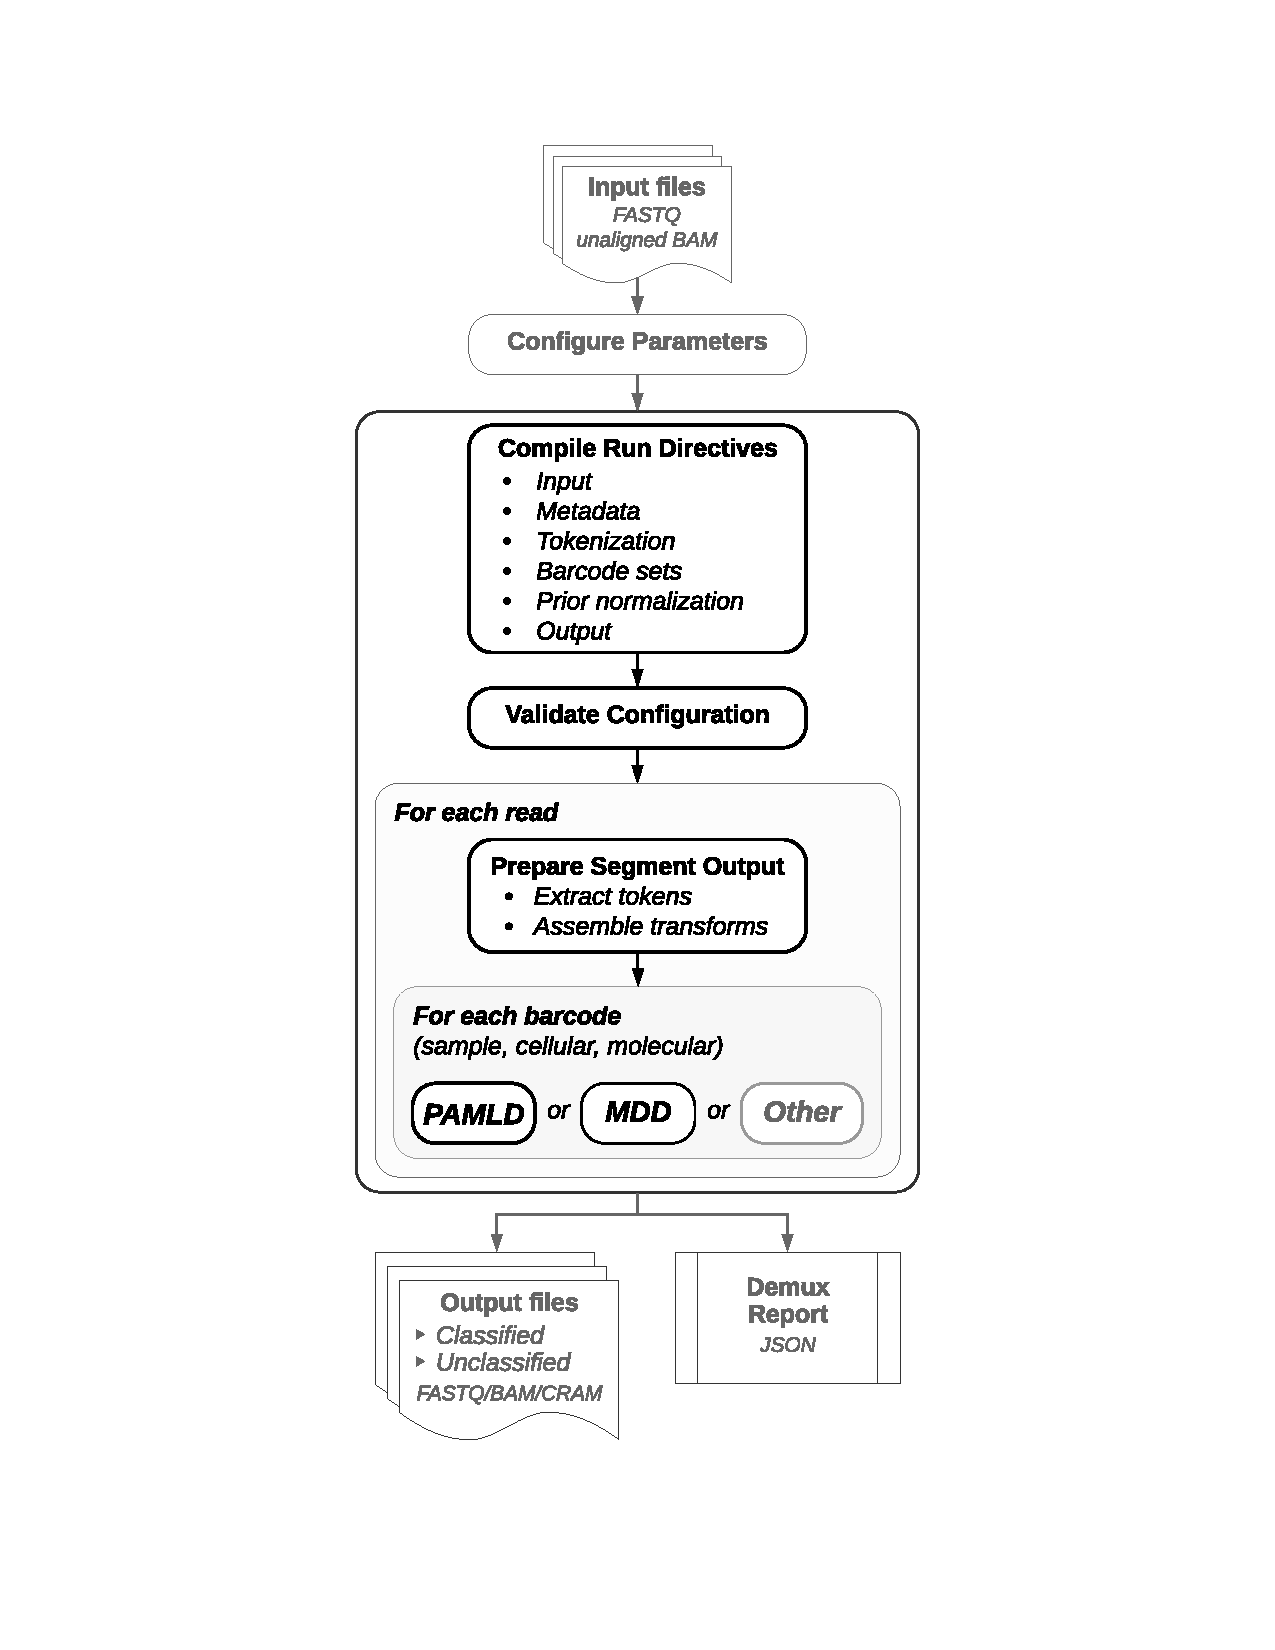
\includegraphics[keepaspectratio,scale=0.5]{pipeline_overview}
\caption{\csentence{Pipeline.} Pheniqs pipeline architecture allowing to easily implement new decoding algorithms.}
\label{fig:02}
\end{figure}

\section*{Results}
%
%
% This should include the findings of the study including, if appropriate, results of statistical analysis which must be included either in the text or as tables and figures. This section may be combined with the Discussion section for Software articles.
% The user interface should be described and a discussion of the intended uses of the software, and the benefits that are envisioned, should be included, together with data on how its performance and functionality compare with, and improve, on functionally similar existing software. A case study of the use of the software may be presented. The planned future development of new features, if any, should be mentioned.

\subsection*{Accuracy analysis with synthetic data}
Since indel errors occur at a much lower rate than substitutions \cite{doi:10.1038/s41598-018-29325-6}, we used a simple model that introduces an error on a nucleobase according to the quality score and substitution frequencies made available with LRSim\cite{doi:10.1016/j.csbj.2017.10.002}. We first paired each read from the run published with deML with a perfect barcode sequence sampled from the estimated prior distribution. To simulate foreign sequences we sampled from a random offset on the \emph{PhiX174} genome. We then generated multiple files with position-independent substitution errors simulated on the barcode bases with quality scores calibrated to increasing error rates.

Each library was evaluated as a binary classifier, so a correct assignment was counted as a true positive ($TP$) while an incorrect assignment was counted as a false negative ($FN$) for the correct library and as a false positive ($FP$) for the incorrectly assigned library. We then summed up the values from all libraries and computed the \emph{precision} ($\frac{TP}{FP + TP}$),  \emph{recall} ($\frac{TP}{FN + TP}$) and \emph{F-score} (harmonic average of the precision and recall). Reads that were marked by either Pheniqs or deML as failing quality control were considered to be unclassified for this analysis.

\subsection*{Prior estimation}
To study the effect of accounting for priors on precision and recall, we estimated the noise prior $P_{\varepsilon}$ and the individual library priors $P(b)$ for each $b \in \mathcal{B}$ from the high confidence reads. Let $S_{\varepsilon}$ be the number of reads filtered by the \emph{noise filter}, $S_{b}$ the number of reads classified to $b$ with confidence higher than $C$ and $S_\mathcal{B} = \sum_{b \in \mathcal{B}} S_{b}$. An estimator for the noise prior is

%
\begin{equation}
\hat{P_{\varepsilon}} = \frac{S_{\varepsilon}}{S_{\varepsilon} + S_\mathcal{B}}
\end{equation}
%

and for an individual barcode is

%
\begin{equation}
\hat{P(b)} = \frac{S_{b}}{S_{\varepsilon} + S_\mathcal{B}}
\end{equation}
%

\begin{figure}[h!]
\centering
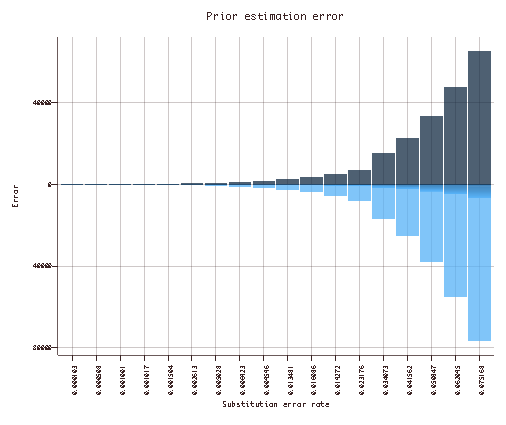
\includegraphics[keepaspectratio,scale=1]{decoder_prior}
\caption{\csentence{Prior estimation error.} Total number of reads misclassified by the prior estimate for individual libraries (shades of blue) or the noise class (gray) are shown as a function of overall error rates. A higher proportion of reads are assigned to the noise class as the error rate increases.}
% \label{fig:03}
\end{figure}

$\hat{P_{\varepsilon}}$ and $\hat{P(b)}$ assume that low confidence reads, i.e. reads that passed the  \emph{noise filter} but failed the \emph{confidence filter}, come from the same distribution. When compared to the true known prior (Figure~\ref{fig:01}) for the simulated data, the error in estimation was negligible for rates lower than 1 per 1000, the expected error rate on most Illumina platforms. Although the error in estimating $\hat{P(b)}$ remained low, the error in estimating $\hat{P_{\varepsilon}}$ grew higher with the error rate due to the difficulty in distinguishing noise from low confidence. This suggests that platforms with high error rates would benefit from prior estimation that accounts for this.

\begin{figure}[h!]
\centering
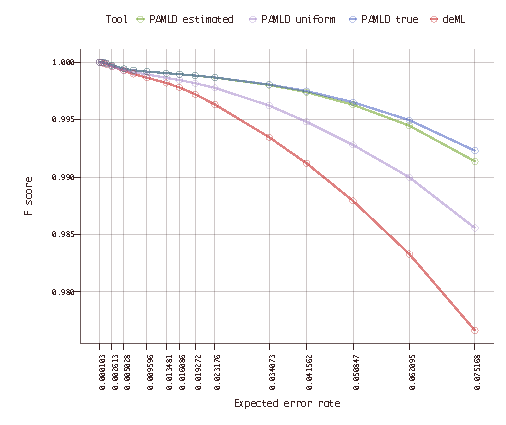
\includegraphics[keepaspectratio,scale=1]{decoder_fscore}
\caption{\csentence{F-Score.} F-score reported for deML and Pheniqs using PAMLD with 3 different priors: true, estimated and uniform.}
\label{fig:04}
\end{figure}

As expected PAMLD performs best with the true prior but only marginally worse with the estimated prior; it performs least well with a uniform prior, as is used by deML. In all 3 cases Pheniqs outperforms deML in both precision and recall (Figure~\ref{fig:02}).

\section*{Conclusion}
%
%
% This should state clearly the main conclusions and provide an explanation of the importance and relevance of the case, data, opinion, database or software reported.

%%%%%%%%%%%%%%%%%%%%%%%%%%%%%%%%%%%%%%%%%%%%%%
%%                                          %%
%% Backmatter begins here                   %%
%%                                          %%
%%%%%%%%%%%%%%%%%%%%%%%%%%%%%%%%%%%%%%%%%%%%%%

\begin{backmatter}

\section*{Competing interests}
  The authors declare that they have no competing interests.

\section*{Author's contributions}
    Text for this section \ldots

\section*{Acknowledgements}
  Text for this section \ldots
%%%%%%%%%%%%%%%%%%%%%%%%%%%%%%%%%%%%%%%%%%%%%%%%%%%%%%%%%%%%%
%%                  The Bibliography                       %%
%%                                                         %%
%%  Bmc_mathpys.bst  will be used to                       %%
%%  create a .BBL file for submission.                     %%
%%  After submission of the .TEX file,                     %%
%%  you will be prompted to submit your .BBL file.         %%
%%                                                         %%
%%                                                         %%
%%  Note that the displayed Bibliography will not          %%
%%  necessarily be rendered by Latex exactly as specified  %%
%%  in the online Instructions for Authors.                %%
%%                                                         %%
%%%%%%%%%%%%%%%%%%%%%%%%%%%%%%%%%%%%%%%%%%%%%%%%%%%%%%%%%%%%%

% if your bibliography is in bibtex format, use those commands:
\bibliographystyle{bmc-mathphys} % Style BST file (bmc-mathphys, vancouver, spbasic).
\bibliography{reference}      % Bibliography file (usually '*.bib' )
% for author-year bibliography (bmc-mathphys or spbasic)
% a) write to bib file (bmc-mathphys only)
% @settings{label, options="nameyear"}
% b) uncomment next line
%\nocite{label}

% or include bibliography directly:
% \begin{thebibliography}
% \bibitem{b1}
% \end{thebibliography}

%%%%%%%%%%%%%%%%%%%%%%%%%%%%%%%%%%%
%%                               %%
%% Figures                       %%
%%                               %%
%% NB: this is for captions and  %%
%% Titles. All graphics must be  %%
%% submitted separately and NOT  %%
%% included in the Tex document  %%
%%                               %%
%%%%%%%%%%%%%%%%%%%%%%%%%%%%%%%%%%%

%%
%% Do not use \listoffigures as most will included as separate files

\section*{Figures}
%   \begin{figure}[h!]
%   \caption{\csentence{Sample figure title.}
%       A short description of the figure content
%       should go here.}
%       \end{figure}
%
% \begin{figure}[h!]
%   \caption{\csentence{Sample figure title.}
%       Figure legend text.}
%       \end{figure}

%%%%%%%%%%%%%%%%%%%%%%%%%%%%%%%%%%%
%%                               %%
%% Tables                        %%
%%                               %%
%%%%%%%%%%%%%%%%%%%%%%%%%%%%%%%%%%%

%% Use of \listoftables is discouraged.
%%
\section*{Tables}
% \begin{table}[h!]
% \caption{Sample table title. This is where the description of the table should go.}
%       \begin{tabular}{cccc}
%         \hline
%            & B1  &B2   & B3\\ \hline
%         A1 & 0.1 & 0.2 & 0.3\\
%         A2 & ... & ..  & .\\
%         A3 & ..  & .   & .\\ \hline
%       \end{tabular}
% \end{table}

%%%%%%%%%%%%%%%%%%%%%%%%%%%%%%%%%%%
%%                               %%
%% Additional Files              %%
%%                               %%
%%%%%%%%%%%%%%%%%%%%%%%%%%%%%%%%%%%

\section*{Additional Files}
  % \subsection*{Additional file 1 --- Sample additional file title}
  %   Additional file descriptions text (including details of how to
  %   view the file, if it is in a non-standard format or the file extension).  This might
  %   refer to a multi-page table or a figure.
  %
  % \subsection*{Additional file 2 --- Sample additional file title}
  %   Additional file descriptions text.


\end{backmatter}
\end{document}
